\section{Analysis}
\label{sec:analysis}
Because the headline 30B result is single-sample, we isolate the decode-time levers
on the 14B, which we can sample freely; all ablations use the same cached samples.

\paragraph{Abstention.}
Abstention matters most exactly where the metric rewards silence. On the three
null-heavy relations, even predicting nothing beats the official 9B baseline
(Section~\ref{sec:task}), so the question is whether a real model does better by
abstaining \emph{selectively} rather than never. It does: decoding the 14B with
consistency voting lifts its null-heavy average from $0.642$ (single sample) to
$0.659$ at $\theta{=}0.5$. The gain is modest but consistent, and it comes from
precision: raising $\theta$ collapses inconsistent (usually wrong) guesses to
$\emptyset$, trading a little recall to suppress false positives.

\paragraph{Setting the threshold.}
How high should $\theta$ be? Figure~\ref{fig:ablate} sweeps it for the 14B on the
null-heavy relations. Our deployed systems fix $\theta{=}0.5$; the sweep is
diagnostic (run on the split we report on, so its optima are optimistic, not tuned
back in). Even so, the pattern argues for per-relation thresholds:
\textsc{personHasCityOfDeath} (39\% empty)
peaks at a low $\theta$ and falls off as voting grows stricter, while
\textsc{countryLandBordersCountry} and \textsc{companyTradesAtStockExchange}
tolerate aggressive voting. Numeric relations are a different story: median
aggregation is roughly neutral, so the gap there is knowledge-bound rather than
variance-bound; the model's area and capacity guesses are often the right order of
magnitude but fall outside the 5\% band (the \textsc{hasArea} miss in
Table~\ref{tab:qual}).

\begin{figure}[t]
\centering
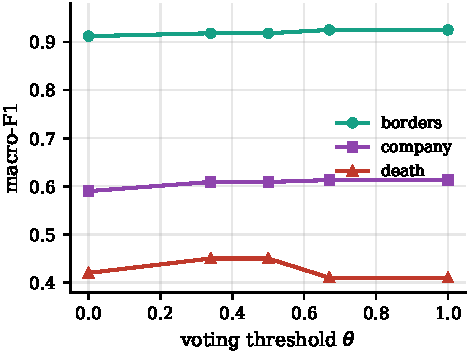
\includegraphics[width=\columnwidth]{figures/fig_ablation.pdf}
\caption{Per-relation validation F\textsubscript{1} vs.\ the voting threshold
$\theta$ (Qwen2.5-14B) on the three null-heavy relations. The most null-heavy
relation (\textsc{death}, 39\% empty) peaks at a low $\theta$ and declines as
voting grows stricter, while borders and company tolerate aggressive voting,
arguing for per-relation thresholds.}
\label{fig:ablate}
\end{figure}

\paragraph{The \textsc{awardWonBy} recall cap.}
The relation \textsc{awardWonBy}, which we beat the baseline on only narrowly, is
recall-capped, and this limit constrains both models. Gold sets average
${\sim}146$ recipients (max 610), but the 14B enumerates only ${\sim}11$ names; its
outputs are \emph{not} truncated, it closes the JSON early, capping recall near
$11/146\approx0.07$. The listed names are often plausible but wrong ($P{=}0.39$).
Parametric recall and a reluctance to enumerate bound this relation; within a
closed-book single model it is largely unsolved, and a larger in-budget model or
multi-step decomposition would help most.

\paragraph{Qualitative behaviour.}
Table~\ref{tab:qual} shows representative Gemma-4-31B outputs: exact on well-known
facts and near-complete on borders, with the two error modes above visible, a
numeric near-miss on \textsc{hasArea} and plausible-but-wrong famous names on
\textsc{awardWonBy}.

\begin{table*}[t]
\centering\scriptsize
\setlength{\tabcolsep}{4pt}
\begin{tabular}{@{}llp{4.2cm}p{4.9cm}c@{}}
\toprule
Relation & Subject & Gold (abbrev.) & Gemma-4-31B output & \\
\midrule
borders & Ethiopia & Djibouti, Eritrea, Kenya, Somalia, S.\ Sudan, Sudan & Djibouti, Eritrea, Kenya, Somalia, S.\ Sudan & \checkmark\,5/6 \\
death & Vito Acconci & New York City & New York City & \checkmark \\
company & Bharti Airtel & Bombay Stock Exch., NSE of India & Bombay Stock Exchange, NSE of India & \checkmark \\
capacity & Gileno de Carli & 5000 & 5000 & \checkmark \\
area & Lo\v{s}inj & 74.36 & 123.3 & $\times$ \\
award & Stockholm hon.\ dr & Torvalds, Hedlund, Trebst, \dots(40) & Mandela, Tutu, Annan, Yunus, \dots & $\times$ \\
\bottomrule
\end{tabular}
\caption{Qualitative examples: Gemma-4-31B vs.\ gold. Exact hits on
\textsc{personHasCityOfDeath}/\textsc{hasCapacity}, near-complete borders; the
numeric near-miss (\textsc{hasArea}) and plausible-but-wrong enumeration
(\textsc{awardWonBy}) are the knowledge-bound errors discussed above.}
\label{tab:qual}
\end{table*}
